\subsection{Equivalence Model}

{
\setbeamertemplate{background canvas}{\tikz[remember picture]\node[opacity=0.7] at (current page.center) {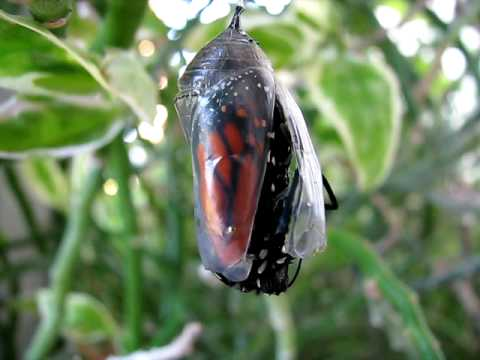
\includegraphics[height=\textheight,keepaspectratio]{nontex/illustrations/emerging.jpg}};}
\begin{frame}
\frametitle{What Different Ways Can A Regex Be Represented?}
\begin{block}{\begin{Large}Regex Equivalence Model Is Missing\end{Large}}
\begin{itemize}
\item \begin{large}regex refactoring is new\end{large}
\item \begin{large}equivalence model required for refactoring\end{large}
\end{itemize}
\end{block}
\end{frame}
}
\note[itemize]{
    \item https://i.ytimg.com/vi/Gt-5lS9hJFA/hqdefault.jpg
}

%------------------------------------------------

\begin{frame}
\frametitle{Regex Equivalence Classes}
\begin{figure}[h]
  \centering
  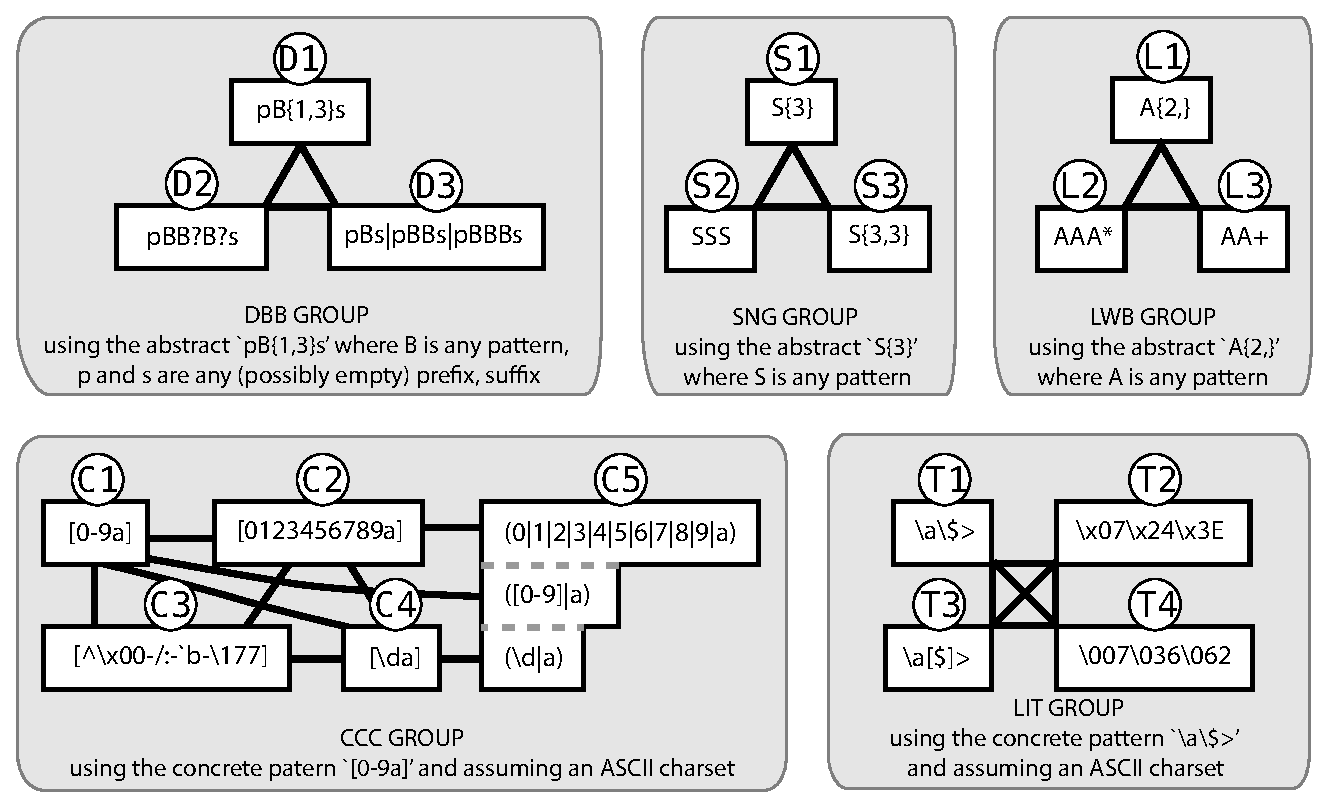
\includegraphics[scale=0.5]{nontex/illustrations/refactoringTree.eps}
  \label{fig:refactoringTree}
\end{figure}
\end{frame}
\note[itemize]{
    \item pt 1
    \item pt 2
}

%------------------------------------------------


\begin{frame}[fragile]
\frametitle{Example Equivalences}
\begin{description}
\item [LIT]: \cverb![\072\073]! $\equiv$ \cverb![}{]!
\item [DBB]: \cverb!((q4f)?ab)! $\equiv$ \cverb!(q4fab|ab)!
\item [CCC]: \cverb!tri[a-f]3! $\equiv$ \cverb!tri(a|b|c|d|e|f)3!
\item [LWB]: \cverb!zaa*! $\equiv$ \cverb!za+!
\item [SNG]: \cverb![aeiou]{2}! $\equiv$ \cverb![aeiou][aeiou]!
\end{description}
\begin{center}
How to decide which representation is preferred?
\end{center}
\end{frame}
\note[itemize]{
    \item in hindsight, different bounds and number of operators should have been treated separately, maybe even different lengths
}

%------------------------------------------------
